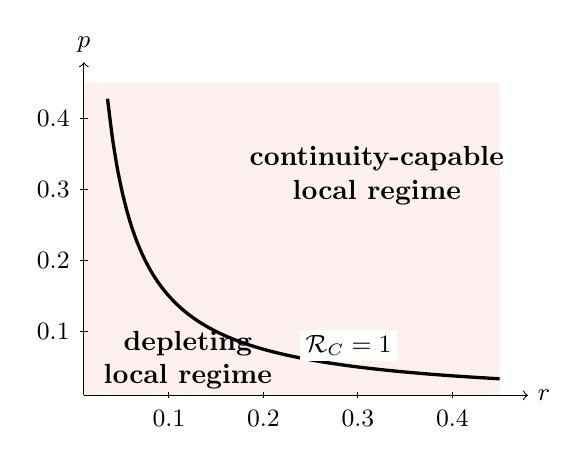
\begin{tikzpicture}[x=12cm,y=9cm,font=\small]
\fill[red!6] (0.01,0.01) rectangle (0.45,0.45);
\fill[green!7] (0.035,0.45) -- (0.03500,0.42857) (0.04019,0.37325) (0.04537,0.33058) (0.05056,0.29666) (0.05575,0.26906) (0.06094,0.24615) (0.06613,0.22684) (0.07131,0.21034) (0.07650,0.19608) (0.08169,0.18363) (0.08687,0.17266) (0.09206,0.16293) (0.09725,0.15424) (0.10244,0.14643) (0.10762,0.13937) (0.11281,0.13296) (0.11800,0.12712) (0.12319,0.12177) (0.12837,0.11685) (0.13356,0.11231) (0.13875,0.10811) (0.14394,0.10421) (0.14913,0.10059) (0.15431,0.09721) (0.15950,0.09404) (0.16469,0.09108) (0.16987,0.08830) (0.17506,0.08568) (0.18025,0.08322) (0.18544,0.08089) (0.19062,0.07869) (0.19581,0.07660) (0.20100,0.07463) (0.20619,0.07275) (0.21137,0.07096) (0.21656,0.06926) (0.22175,0.06764) (0.22694,0.06610) (0.23212,0.06462) (0.23731,0.06321) (0.24250,0.06186) (0.24769,0.06056) (0.25287,0.05932) (0.25806,0.05813) (0.26325,0.05698) (0.26844,0.05588) (0.27363,0.05482) (0.27881,0.05380) (0.28400,0.05282) (0.28919,0.05187) (0.29437,0.05096) (0.29956,0.05007) (0.30475,0.04922) (0.30994,0.04840) (0.31512,0.04760) (0.32031,0.04683) (0.32550,0.04608) (0.33069,0.04536) (0.33587,0.04466) (0.34106,0.04398) (0.34625,0.04332) (0.35144,0.04268) (0.35662,0.04206) (0.36181,0.04146) (0.36700,0.04087) (0.37219,0.04030) (0.37738,0.03975) (0.38256,0.03921) (0.38775,0.03868) (0.39294,0.03817) (0.39812,0.03768) (0.40331,0.03719) (0.40850,0.03672) (0.41369,0.03626) (0.41887,0.03581) (0.42406,0.03537) (0.42925,0.03494) (0.43444,0.03453) (0.43962,0.03412) (0.44481,0.03372) (0.45000,0.03333) -- (0.45,0.45) -- cycle;
\draw[->] (0.01,0.01) -- (0.48,0.01) node[right] {$r$};
\draw[->] (0.01,0.01) -- (0.01,0.48) node[above] {$p$};
\foreach \x in {0.1,0.2,0.3,0.4} {\draw (\x,0.006)--(\x,0.014) node[below=3pt] {\x};}
\foreach \y in {0.1,0.2,0.3,0.4} {\draw (0.006,\y)--(0.014,\y) node[left=3pt] {\y};}
\draw[very thick] plot[smooth] coordinates {(0.03500,0.42857) (0.04019,0.37325) (0.04537,0.33058) (0.05056,0.29666) (0.05575,0.26906) (0.06094,0.24615) (0.06613,0.22684) (0.07131,0.21034) (0.07650,0.19608) (0.08169,0.18363) (0.08687,0.17266) (0.09206,0.16293) (0.09725,0.15424) (0.10244,0.14643) (0.10762,0.13937) (0.11281,0.13296) (0.11800,0.12712) (0.12319,0.12177) (0.12837,0.11685) (0.13356,0.11231) (0.13875,0.10811) (0.14394,0.10421) (0.14913,0.10059) (0.15431,0.09721) (0.15950,0.09404) (0.16469,0.09108) (0.16987,0.08830) (0.17506,0.08568) (0.18025,0.08322) (0.18544,0.08089) (0.19062,0.07869) (0.19581,0.07660) (0.20100,0.07463) (0.20619,0.07275) (0.21137,0.07096) (0.21656,0.06926) (0.22175,0.06764) (0.22694,0.06610) (0.23212,0.06462) (0.23731,0.06321) (0.24250,0.06186) (0.24769,0.06056) (0.25287,0.05932) (0.25806,0.05813) (0.26325,0.05698) (0.26844,0.05588) (0.27363,0.05482) (0.27881,0.05380) (0.28400,0.05282) (0.28919,0.05187) (0.29437,0.05096) (0.29956,0.05007) (0.30475,0.04922) (0.30994,0.04840) (0.31512,0.04760) (0.32031,0.04683) (0.32550,0.04608) (0.33069,0.04536) (0.33587,0.04466) (0.34106,0.04398) (0.34625,0.04332) (0.35144,0.04268) (0.35662,0.04206) (0.36181,0.04146) (0.36700,0.04087) (0.37219,0.04030) (0.37738,0.03975) (0.38256,0.03921) (0.38775,0.03868) (0.39294,0.03817) (0.39812,0.03768) (0.40331,0.03719) (0.40850,0.03672) (0.41369,0.03626) (0.41887,0.03581) (0.42406,0.03537) (0.42925,0.03494) (0.43444,0.03453) (0.43962,0.03412) (0.44481,0.03372) (0.45000,0.03333)};
\node[align=center,font=\bfseries] at (0.32,0.32) {continuity-capable\\local regime};
\node[align=center,font=\bfseries] at (0.12,0.06) {depleting\\local regime};
\node[fill=white,inner sep=2pt] at (0.29,0.08) {$\mathcal{R}_C=1$};
\end{tikzpicture}
